\section{Requirements}
\subsection{Background}
Requirements elicitation is a very difficult part of software development. In order to understand what requirements elicitation is, we first have to further define requirement:
\begin{quote}
	(1) a condition or capability needed by a user to solve a problem or achieve an objective; (2) a condition or capability that must be met or possessed by a system or system component to satisfy a contract, standard, specification, or other formally imposed documents; (3) a documented representation of a condition or capability as in (1) or (2)\cite{september1990ieee}.
\end{quote}
In game design, many of the users requirements are vague and subjective. For example, the requirement that a game must be \emph{fun} and \emph{absorbing} is not a very well understood requirement. 

Also, the exact breakdown of what requirements elicitation entails is still being debated. Once source separates requirements into function and nonfunctional requirements\cite{southwell1987requirements}. They then further classify the nonfunctional requirements into performance/reliability, interfaces, and design constraints.

The process for requirements elicitation is decomposed into three activities \cite{rzepka1989requirements}. The first is the elicitation of requirements from various individual sources. Then you need to insure that the needs of all users are consistent and feasible, and finally you need to validate that the requirements are an accurate reflection of the users needs.

There are many general problems with elicitation including\cite{mcdermid1989requirements}:
\begin{enumerate}
	\item Problems of scope
	\begin{itemize}
		\item The boundary of the system is ill-defined
		\item Unnecessary design information was given
	\end{itemize}
	\item Problems of understanding
	\begin{itemize}
		\item Users have incomplete understanding of their needs
		\item Users have poor understanding of computer capabilities
		\item Analysts have poor knowledge of problem domain
		\item User and analyst speak different languages
		\item Ease of omitting ``obvious'' information
		\item Conflicting views of different users
		\item Requirements are often vague and untestable, e.g. ``user friendly'' and ``robust''
	\end{itemize}
	\item Problems of volatility
	\begin{itemize}
		\item Requirements evolve over time
	\end{itemize}
\end{enumerate}
The understanding and volatility issues will still be present in game design, but scope issues may not be as large of a problem as they are in other software systems.

\subsection{Requirements Documents}

The requirements elicitation process usually requires a game design document, written by the game design team. The design document is usually less formal than a typical software design document\cite{callele2005requirements}. This is partially due to the fact that the imposition of too much structure can be detrimental to the creative process. The game design document is usually used as the requirements document as defined by the preproduction team\cite{callele2005requirements}. 

A game design document should describe several things\cite{bethke2003game}
\begin{itemize}
	\item \emph{Define the game:} Articulate what the game is as clearly as possible
	\item \emph{Core Gameplay:} Describe the main view, player activity, the user interface
	\item \emph{Contextual Gameplay:} Shell menus, tutorial mechanics, multiplayer mechanics
	\item \emph{Talk Story:} Describes the world backstory, character backgrounds, the levels, missions
	\item \emph{Game Assets:} Design of the 3D models, voices, motion capture, sound effects, music
\end{itemize}

The requirements documents are usually written along side the design documents. Requirements can take several forms including\cite{bethke2003game} frame rate requirements, the size of the resulting binary, the length of time it should take to product the product, having few defects, being able to process 100,000 polygon characters, etc. Once as many of the requirements as possible have been identified, the requirements are usually modelled using UML and use case diagrams as in standard software engineering. Prototyping is also very common, figure \ref{mockup} shows a mockup in early production, and \ref{final} shows the resulting screen. 

\begin{figure}[!ht]
	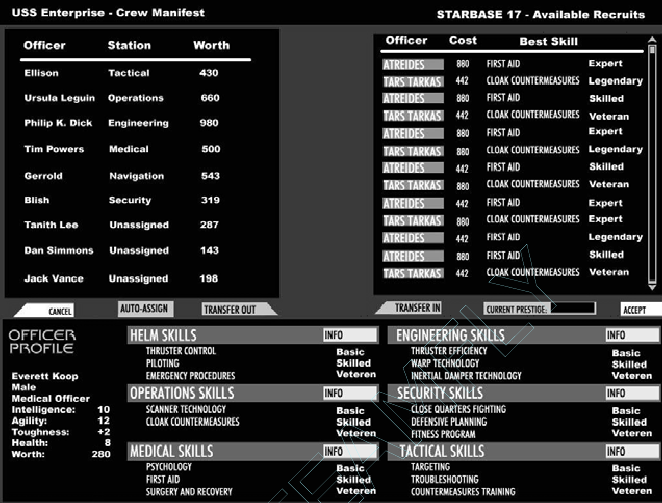
\includegraphics[scale=0.5]{Images/mockup}
	\label{mockup}
	\caption{Mockup early in production \cite{bethke2003game}}
\end{figure}

\begin{figure}[!ht]
	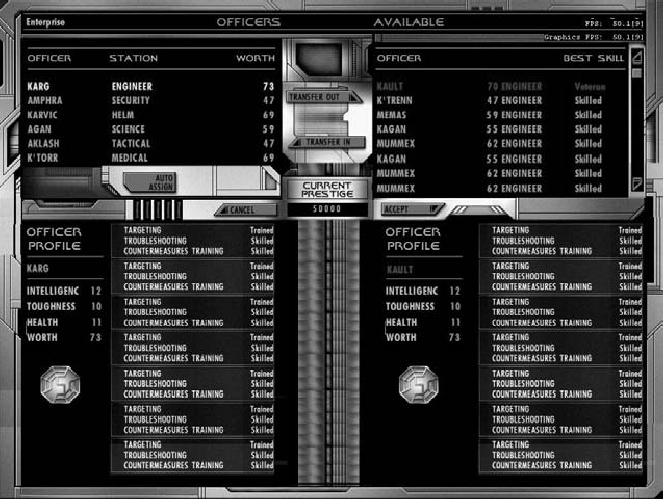
\includegraphics[scale=0.5]{Images/final}
	\label{final}
	\caption{Production screen \cite{bethke2003game}}
\end{figure}

\subsection{Emotional Requirements}

Once of the most difficult parts of requirements elicitation process is the specification of the emotional requirements. Video game designers are concerned with the players experience which is rather difficult to define. One definition describes the player experience as ``the means by which the player's consciousness is cognitively engaged while simultaneously inducing emotional responses''\cite{callele2006emotional}. The emotional requirements can then be further broken down into the emotional intent of the designer and the means by which the designer expects to induce the target emotional state\cite{callele2006emotional}. This makes the nonfunctional requirements much more paramount to the success of the software system. In order to successfully capture the emotional requirement, it must capture ``the intent of the designer, and the means by which the designer expects to induce the target emotional state''\cite{callele2006emotional}.

There are several different methods for representing emotional requirements. The \emph{emotional terrain} method captures artistic expression with spatial qualifiers. A range of colors are used in order to represent emotion at a specific point in time in a game. A newer method requires creating an \emph{emotion intensity map} (Figure \ref{emotion_intensity_map}).

\begin{figure}[!ht]
	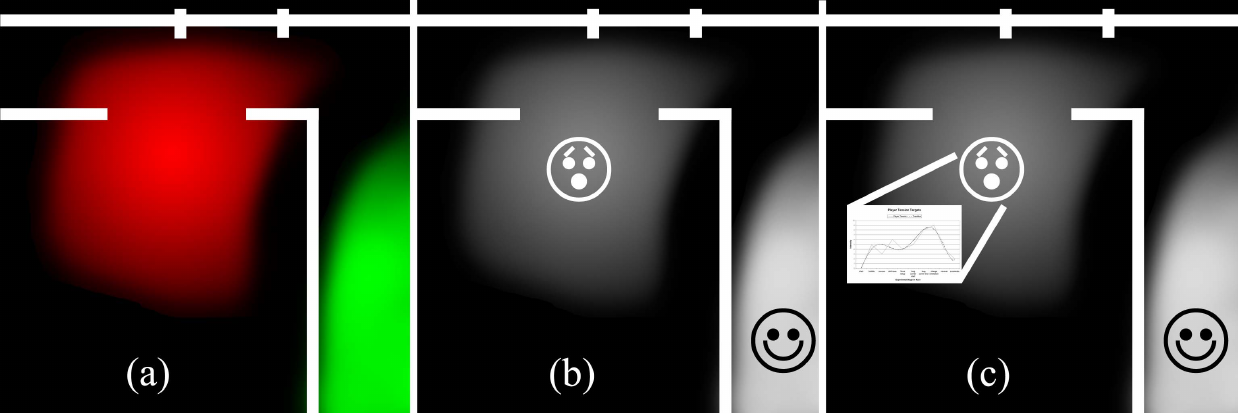
\includegraphics[scale=0.27]{Images/emotion_intensity_map}
	\label{emotion_intensity_map}
	\caption{Emotion Intensity Map \cite{callele2006emotional}}
\end{figure}

The emotion intensity map uses luminance to quantify intensity, and emotions are mapped by either a Chernoff Face\cite{flury1981graphical}, or Ekman's Facial Action Coding System\cite{ekman2002facial}.

\emph{Temporal qualifiers} are also unique to game design. For example, ``if a player reaches a room within 5 minutes of the start of gameplay, the player is very skilled so increase the intensity''\cite{callele2006emotional}. Focus groups and post-gameplay interviews can also be used to gauge the emotional response of the users during gameplay. This can be used to ensure that the desired emotion is induced in the user at the correct time in a game.

There are also several software requirements that are never captured in an official manner\cite{bentley2002putting}. In practice, usability, immersion, and motivation are usually considered in user surveys.

\section{Design}

\subsection{Background}
As with most software industries, when the paradigm of programming of software designs shifted from imperative to object-oriented programming, the game development industry adopted this change to take advantage of the many benefits that it offered. These benefits included data encapsulation, easier mapping of concepts to programming structures, and the ability to group and share behavior amongst objects of the same functional type. These benefits allowed additional functionality to be inserted without the need to duplicate a lot of code, thus greatly reducing the time, effort, and cost of developing large-scale software products.

\begin{figure}[h!]
  \centering 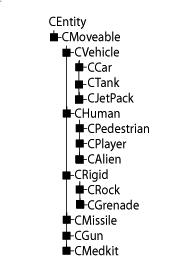
\includegraphics[width=0.2\textwidth]{Images/tree}
  \caption{A typical game object hierarchy. \cite{west2006evolve}}
\end{figure}

In a typical object-oriented software product, the objects form a hierarchical tree that has width (many objects with the same direct ancestor, such as there are many weapon-types that are each modeled as an object, and they would all share the same ancestor of 'Weapon'), and height (set of objects that form a list of direct ancestors for each other, such as how a 'DwarfMale' is a 'Dwarf' that is a 'PlayableCharacter' that is a 'Character' that is an 'Entity', and so on). This tree-like structure describes the term inheritance, where one object such as 'DwarfMale' may inherit functionality from 'Dwarf'. In small-to-medium sized products, inheritance can make development both simpler and much more efficient. However, as projects grow and changes are made, designing objects around inheritance can lead to problems due to relationships between objects in the tree. Changing or adding code at the root of the tree may cause the changes to cascade down through the rest of the tree, resulting in undesired behavior, as described by Herb Marslas, a developer for Age of Empires II:

\begin{quote}
\ldots functionality can be added or changed in a single place in the code to affect many different game units. One such change inadvertently added line-of-sight checking for trees\cite{wilson2003game}.
\end{quote}

With the development archetype shifting from the waterfall method, where projects are defined at the beginning and are less adaptable to changes, to a more agile and iterative-based approach, the ability to change the project on both small and large scales becomes a requirement of the design of the project. As teams in the game development industry began to conduct agile development processes, they began to realize that the object-oriented design paradigm was not as flexible and adaptable as it needed to be, largely in part due to the inheritance structure and requirement of defined interfaces between objects.

To solve the issues with large inheritance trees, architects, designers, and programmers discovered\cite{haller2002generic} the benefits of composition over inheritance, where it is better and/or easier to consider a has-a relationship over an is-a relationship between objects. An example of this can be described as the difference between a 'Character' object having a position in the world, rather than a 'Character' object being a 'PositionalObject'. The distinction is small conceptually, but rather large in terms of design and implementation of the project. In order to change the 'Character' to not having a position, a developer would simply have to remove the position with respect to the composition method, while the inheritance method would require the object to be placed somewhere else in the tree, potentially leading to side effects and/or undesired behavior.

The realization of the benefits of composition over inheritance began a movement of the game development industry to a design pattern known as 'Entity-Component Systems', where objects are modelled by what they are composed of or contain, rather than their position in the hierarchical inheritance tree.

\subsection{Entity-Component Design}

\begin{figure}[h!]
  \centering 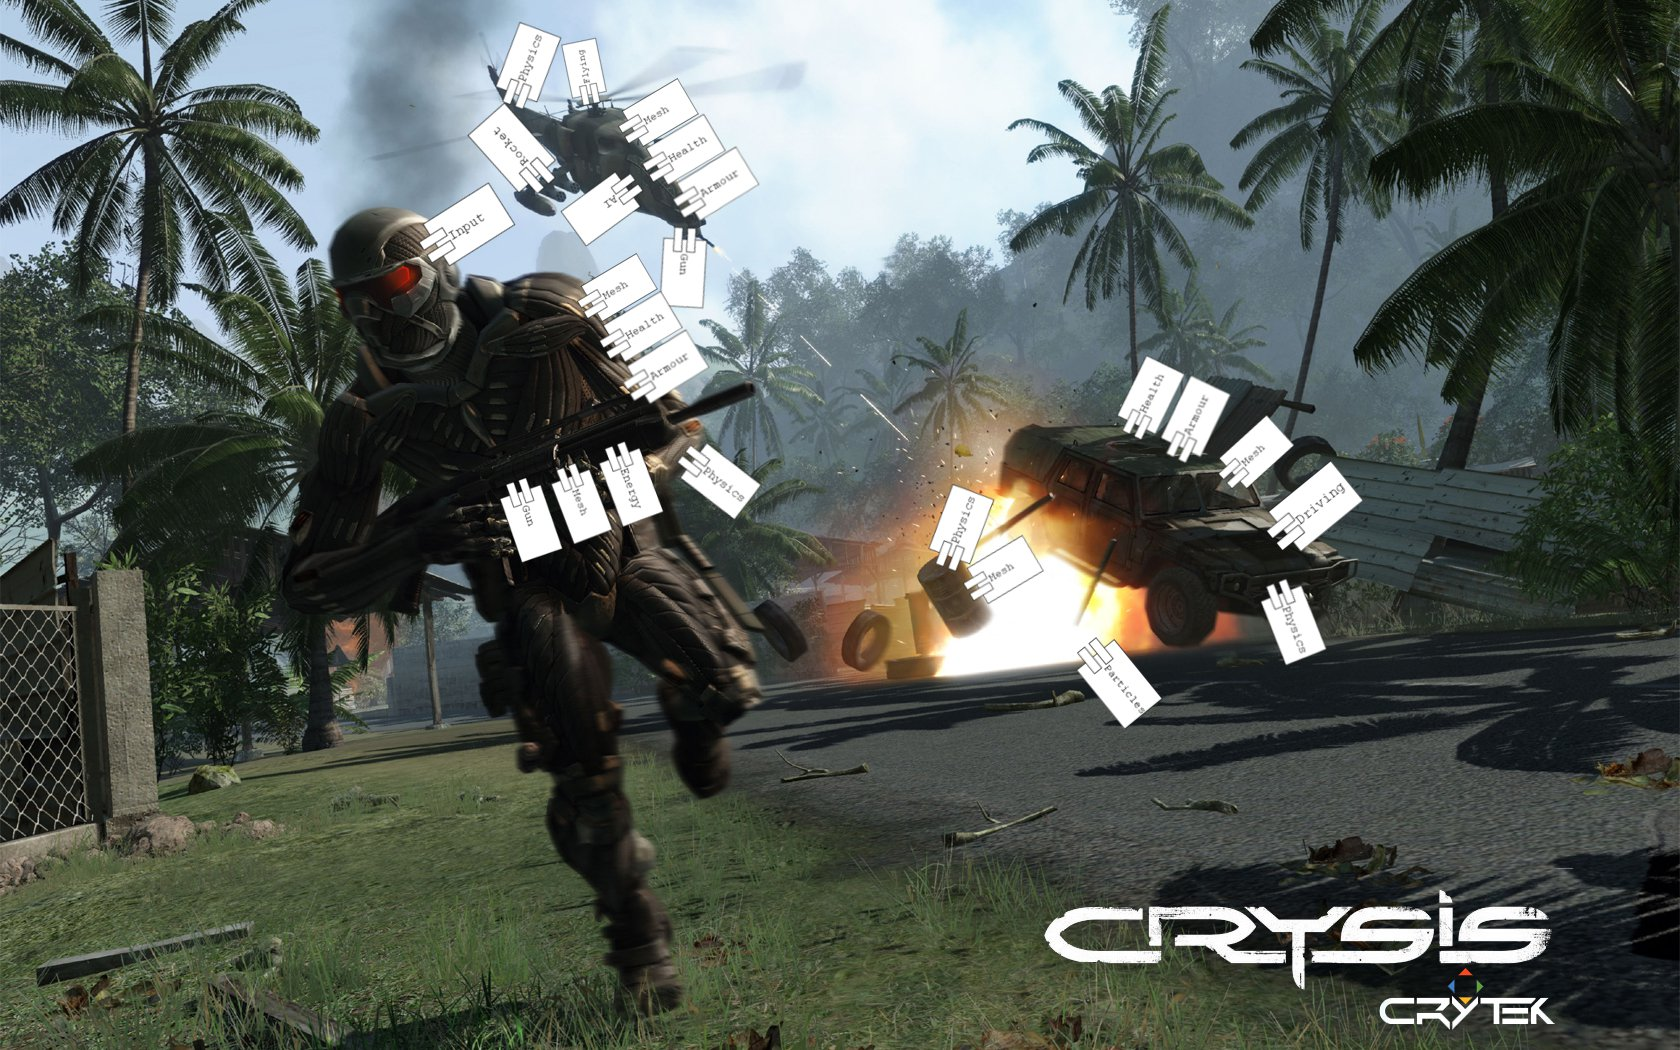
\includegraphics[width=0.48\textwidth]{Images/crysis-components.jpg}
	\caption{Entity component modelling in Crysis. Source: \url{http://piemaster.net-content.s3.amazonaws.com/wp-content/uploads/crysis-components.jpg}}
\end{figure}

The entity-component design paradigm is primarily focused on three primary objects in the application: entities, components, and system-managers (or component-managers). Entities are the primary conceptual objects in the game, such as 'Player', 'Target', and 'Map', among others. Components, on the other hand, are essentially atomic parameters that can be attributed to an entity. For example, a 'Player' entity may have a 'Position' component, a 'Render' component, a 'Velocity' component, a 'Physics' component and anything else that describes the behavior of a 'Player' entity. The other object type, system-managers are objects responsible for the management of entities and their components, and the coordination and synchronization of each respective type. For example, a 'RenderSystemManager' may be responsible for iterating through every entity with a 'Render' component, and rendering that entity to the display.

There are many benefits that this type of design provides. The primary benefit, however, may be the fact that this type of design is inherently agile in nature. Changing the system is simply the process of adding, removing, or editing the desired entities and/or components. For example, to create a hidden trap object, an invisible object in the game that reacts in some way to the player, a developer may simply have to create the 'Trap' entity, provide it with a 'Position' component, and a 'Script' component that provides some behavioral functionality based on the 'Position' of the entity relative to the player, and register the entity with the correct system-manager that can update the 'Script' component whenever the player moves. Or to make the player invisible, a developer could simply remove the 'Render' component from the 'Player' entity. Additionally, once a component has been created, it is possible to reuse the component across the rest of the system or in future projects as it is simply a set of parameters containing no side-effects or requiring any interfaces for any other objects.

\begin{figure}[h!]
  \centering 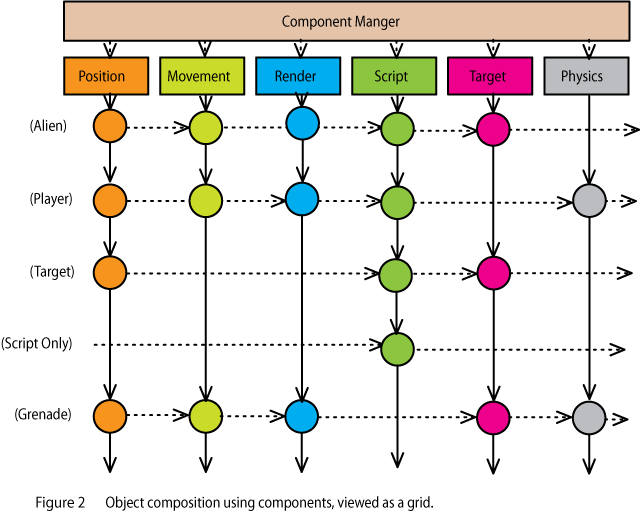
\includegraphics[width=0.5\textwidth]{Images/aggregation.png}
  \caption{Entity-component relationship.\cite{evolve_your_hierarchy}}
\end{figure}

Looking at this type of design, it is clear that the system and all of its entities are data-driven in nature. Rather than an object inheriting from some 'Renderable' object, the desire to render the object is encapsulated into whether or not the entity has a 'Render' component. With this in mind, the complimentary relationship between agile development and entity-component design actually increases due to the fact that rather than having to receive requirements from a customer (the game designer, in respect to the game developer), the developer may actually allow the customer themselves to implement the desired functionality through a scripting engine, such as Dungeon Seige's scripting language Skrit.

\begin{figure}[h!]
  \centering 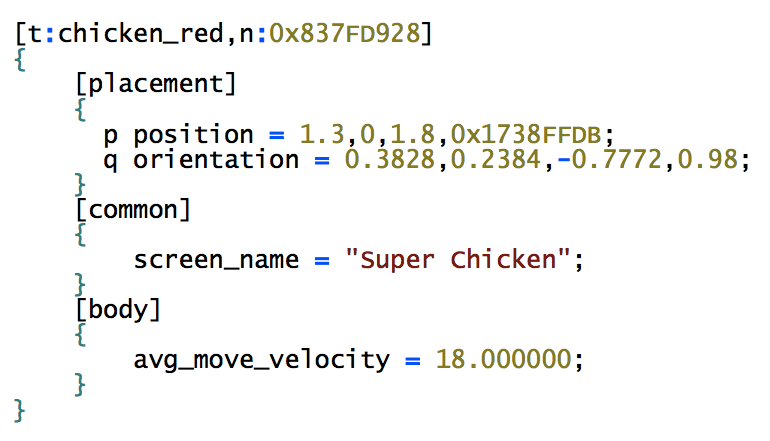
\includegraphics[width=0.4\textwidth]{Images/skrit.png}
	\caption{The Skrit scripting language for describing components in Dungeon Seige II\cite{bilas2002data}.}
\end{figure}

Incorporating scripting languages allows the game designers--that is, the department whose job it is to define the functionality of the game and its entities--to actually define the functionality of an entity. Not only does this align perfectly with the agile manifesto, where interaction with the customer is paramount, but it also (if implemented correctly) allows different entities and components to be injected, removed, or edited at run-time to provide instant feedback to both the developer and the designer. This allows for an efficient iterative approach to be taken when developing the game as a whole.

The combination of entity-component systems with built-in scripting engines has become the primary design paradigm of modern game development, as showcased by the primary free, open source, and production game engines in the market today such as the Unreal Development Kit with Unrealscript scripting, and Unity3D with Mono, C\#, and Javascript scripting.

\subsection{Future of Game Design}

With the increased practice of agile development methodologies, and the realization of its complimentary nature with entity-component design with embedded scripting, it is likely that entity-component systems will continue to be the primary design archetype for the foreseeable future. So where does the industry go from here? A good modification candidate to the current methodology appears to be incorporating functional programming considerations within the game design. Functional programming is a programming method that strives for pure, non-state mathematical functions. Simply speaking, a pure function is a function that receives some input, performs some calculations, and returns a result or a modified copy of the input. A pure function is never able to access any state outside of the function's local scope. This is in stark contrast to the current paradigm of imperative programming, where typically it is the state of the application or an object that determines how the application behaves, with the goal of most functions to put the object or application into some known state.

Functional programming was originally introduced with LISP in the 1950s, but was slowly overshadowed by imperative programming due to the lack of computational resources available to facilitate pure functional programming in performance-critical applications. However, as innovations in the number of transistors able to be packed onto a single processing chip have begun to slow, processors have begun to incorporate additional parallel cores to increase processing power capabilities. With this plateau in processing power per core, and an increasing number of available cores, it is necessary for software to take advantage of parallel, multithreaded computing. However, the current method of imperative programming where application behavior is primarily driven by objects modifying state begins to break down in parallel environments as you begin to require transaction-based state modifications which can impose performance-limiting overhead. Thus, with parallel architectures becoming much more common, a paradigm-shift back to functional programming begins to provide tantalizing benefits.

While functional-versus-imperative programming is primarily an implementation-level decision, understanding the advantages and limitations of functional programming at a design-level may provide a better design in which to implement the specific programming archetype. Additionally, understanding that pure-functions do not interact with program state and do not produce any side effects allows functionality to be created iteratively in an agile approach. It is simply a matter of replacing a pure-function with a new implementation--say a better algorithm or different behavior altogether--and the rest of the code (in terms of program state) is unaffected by unsuspected side effects. With the nature of the code being simpler due to the reduced complexity of program state, the application becomes much easier to maintain and extend.

\section{Testing}

Game developers invest thousands of dollars into testing in order to ensure that the game is designed and tested well enough that it doesn't frustrate the players who purchase the game. Console games in particular have to be tested very thoroughly because it may not be possible to fix bugs after the game has been deployed. Video game testing is very different from testing conventional software systems. The developer wants to immerse the user in their game, and this immersion can be broken by very small bugs in a game. The most common software testing methods are described below, and attempt to address the problem of software bugs.

\subsection{Functionality Testing} Functionality testing is the most common type of testing and can be completed by someone with little or no technical knowledge. Functionality tests can be released to the public or individuals who will then perform the testing for the publisher. These tests check for general problems in a game and the games user interface. These tests primarily deal with issues relating to stability, game mechanics, and the overall integrity of the game. Functionality testing is employed when the game is playable to some degree, but is not ready for a full release.

\subsection{Compliance testing} Compliance testing deals with the general standards for each platform that a game would be released on. Such standards include handling of error messages, copyright material, trademarks, and data persistence. If the game does not meet the standard guidelines as laid out by the platform developer then game will be delayed and costs will increase as a result.

\subsection{Compatibility testing} Compatibility testing tests the game to see if it is compatible with the software and hardware supplied by the publishers. Compatibility testing is used early in the beta version and at the end of the production of the game. This ensures that the hardware includes the brands of several different manufactures and different input devices including joysticks. They also test the performance and results when the hardware is ran at the advertised minimum requirements.

\subsection{Multiplayer testing} Multiplayer testing is used when you have to test a game with multiplayer features. Testing is done to ensure all the connectivity methods, such as modem, LAN, and internet, are working correctly. Online player interaction and proper game performance while online is the main focus of this type of testing.

\subsection{Localization testing} Localization testing deals with checking proper translation of in-game text or dialogue. These testers are usually people who speak multiple languages and understand regional differences between countries.

\subsection{Soak testing} Soak testing tests how the game is running on the system for prolong periods of times in different modes of the operation or during repetitive actions. The modes of operation include pausing the game in various modes of play, remaining on the title screen, or just idling. Usually since this type of testing requires no interaction besides the initial set-up automated tools are used to do any repetitive tasks such as mouse-clicking or button pressing. It is most commonly used to find any memory leaks and rounding errors.

\subsection{Regression testing} Regression testing comes into play when a bug has been found and has been potentially fixed. QA testers must verify that the patch has actually fixed the problem. They must also determine if the fix had a detrimental effect on the game or caused an old bug to resurface.

\subsection{Beta testing} Initial versions of the software are released to the general public or select individuals so that they can physically play the software and find any bugs the testers have missed. This increases the chances of finding bugs in the game itself and is a cheap and efficient way to create hype for the game. Since the game is in beta the players understand that there will be bugs in the game.

\section{Creative Interaction}

\section{Frameworks}

\subsection{Background}
In the game development industry today, Game Engines provide the necessary frameworks, API's, and SDK's for developers to build games for various platforms. The purpose of a game engine is to abstract out the details of commonly used tasks and separate them into reusable components for the developers. Some of the functionality provided by game engine's include Rendering, Physics, User Input, Collision Detection, and Animation. As there are hundreds of different game engines available on the market, functionalities provided by each game engine will differ depending on the type of engine the developers choose to use. There are both commercial and open source game engines but the majority require a commercial license but may include a free non-commercial version.

\subsection{Types of Game Engines}
There are various types of game engines available to developers. At the lowest level, developers will combine many different API's to develop their own game engines. While this gives developers the flexibility of choosing their own components, it usually comes with a drawback of high costs. There can also be technical issues that can arise when trying to use many different libraries together for the first time. The drawbacks associated with this approach make it less attractive in the gaming industry.\\

The mid-level game engines include many features out of the box. These game engines are usually ready for rendering, physics, user interface, collision detection, and much more with less setup required than that of the low level approach. Developers will still need to do a bit of programming to have a complete game up and running. The Unreal Engine 3 is an example of mid-level engines.\\

At the highest level are game engines that allow for point and click game development with very little programming required. Unity3D and GameMaker are examples of this type of game engine which makes the development process as user friendly as possible. Although these are easy to use engines, they come with a drawback. Most of them are limiting in the types of games they can make or the quality of graphics they can produce. The advantage of quickly developing games have made the high level engines more common today.
 
\subsection{Unreal Engine 3}
The Unreal Engine 3 is a cross platform game development toolkit that was developed by Epic Games. This toolkit is widely used by many game developers including BioWare (EA), 2K Games, Epic Games (Microsoft), Arkane Studios (Bethesda Softworks), and many more. It has been used to produce hit games including Gears of War, Borderlands, and BioShock. Epic Games describes the Unreal Engine 3 to have been designed with

\begin{quote}
\ldots ease of content creation and programming in mind, with the goal of putting as much power as possible in the hands of artists and designers to develop assets in a visual environment with minimal programmer assistance, as well as giving programmers a highly modular, scalable and extensible framework for building, testing, and shipping games in a wide range of genres. \cite{unreal_engine_3}
\end{quote}

Features include tools for Animation, Artificial Intelligence, Audio, Physics, Rendering, Networking, and many more. Although the Unreal Engine 3 is a commercial use game engine, Epic Games released the Unreal Development Kit (UDK) which includes many of the features of the Unreal Engine 3 for free non-commercial use.

\begin{figure}[h!]
  \centering 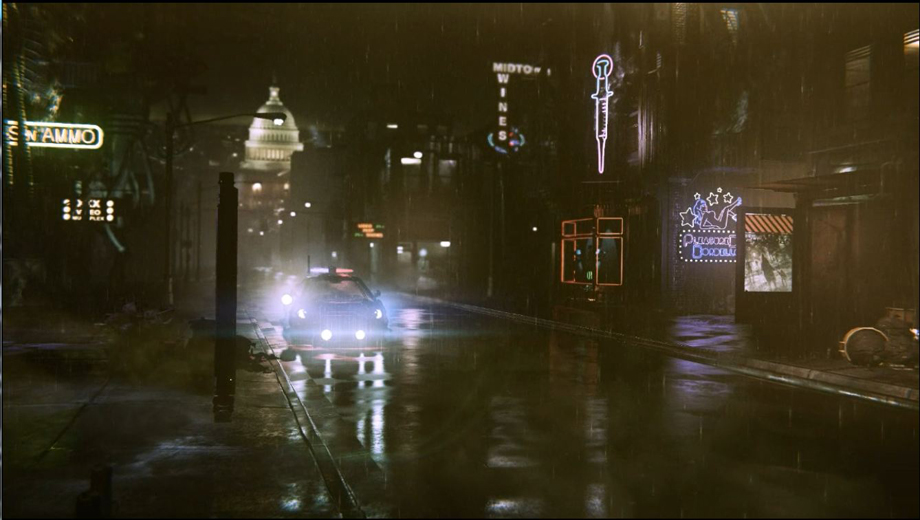
\includegraphics[width=0.48\textwidth]{Images/unreal_engine3_rendering.jpg}
	\caption{Rendering produced using the Unreal Engine 3. Source: \url{http://www.unrealengine.com/files/features/rendering1.JPG}}
\end{figure}

\subsection{CryENGINE 3}
The CryENGINE 3 was developed by Crytek and is used to develop games for Xbox 360, Playstation 3, Windows, and Wii U. CryENGINE 3 was used to develop the first person shooter franchise titled Crysis developed by Crytek and publish by Electronic Arts. Similar to the Unreal Engine 3, CryENGINE 3 is a commercial Game Engine that offers a free version of the toolkit for non-commercial use only. It also includes a large number of tools for Visuals, Characters, AI Systems, Physics, Performance, and many more.
\begin{figure}[h!]
  \centering 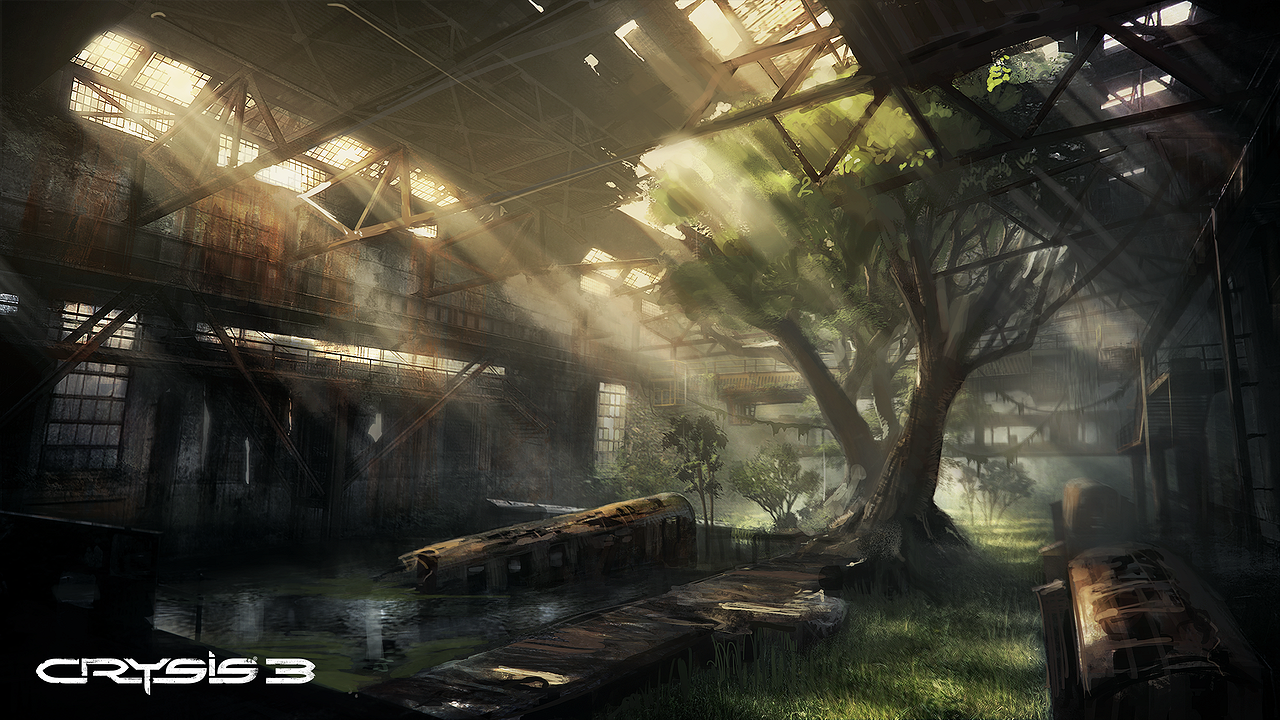
\includegraphics[width=0.48\textwidth]{Images/Crysis3_Fields_Warehouse_ConceptArt.png}
	\caption{Crysis 3 was develop by Crytek using the CryENGINE 3. Source: \url{http://www.crysis.com/us/screenshots/crysis-3-concept-art-warehouse}}
\end{figure}

\subsection{Unity3D}
Unity3D is a cross platform game Engine that can be used for Developing Games for Xbox 360, Playstation 3, Windows, iOS, Android, Mac, and more. Unlike CryENGINE 3 and Unreal Engine 3, Unity has a free version that can be used for developing games for commercial use (with certain conditions). The Pro version of Unity3D has a licensing fee but includes a larger set of features than that of the free version. The developers of Unity call it a 
\begin{quote}
game development ecosystem: a powerful rendering engine fully integrated with a complete set of intuitive tools and rapid workflows to create interactive 3D content; easy multi-platform publishing; thousands of quality, ready-made assets in the Asset Store and a knowledge-sharing Community. \cite{unity3d}
\end{quote}
Although Unity has not been used to produced big name titles like the Unreal Engine 3 has, it is still a popular choice especially for mobile application development. Of the featured games provided on the Unity website, a majority of the titles were developed for iOS, and Android devices.
\begin{figure}[h!]
  \centering 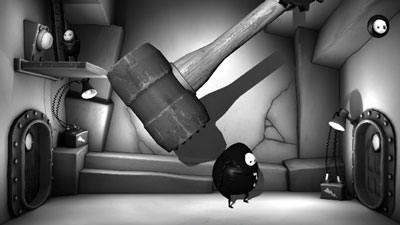
\includegraphics[width=0.48\textwidth]{Images/Escape-plan-screenshot.jpg}
	\caption{"Escape Plan" Developed using Unity3D for the Playstation Vita. Source: \url{http://en.wikipedia.org/wiki/File:Escape-plan-screenshot.jpg}}
\end{figure}

\subsection{Cocos2D}
Cocos2D is an open source 2D game framework released under the MIT License making it free to use and develop for commercial purposes. It has been ported to many different devices including iOS, Android, Blackberry 10, and Windows. There have been thousands of titles produced for mobile devices using Cocos2D.  Unlike Unreal Engine 3, CryENGINE 3, and Unity3D, Cocos2D is not considered a game engine. Its goal is to abstract the details of the low level graphics packages and make game development fast and easy to use for mobile developers. 
\begin{figure}[h!]
  \centering 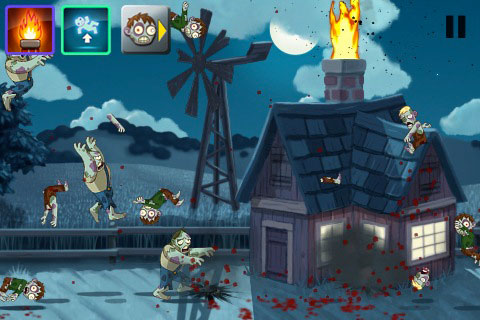
\includegraphics[width=0.48\textwidth]{Images/zombie-smash-screenshot.jpg}
	\caption{"Zombie Smash" Developed for iOS and Android using Cocos2D. Source: \url{http://www.blogcdn.com/www.tuaw.com/media/2010/03/zombie-smash.jpg}}
\end{figure}
